%%%%%%%%%%%%%%%%%%%%%%%%%%%%%%%%%%%%%%%%%%%%%%%%%%%%%%%%%%%%%%%%%%
%%%%%%%% ICML 2016 EXAMPLE LATEX SUBMISSION FILE %%%%%%%%%%%%%%%%%
%%%%%%%%%%%%%%%%%%%%%%%%%%%%%%%%%%%%%%%%%%%%%%%%%%%%%%%%%%%%%%%%%%

% Use the following line _only_ if you're still using LaTeX 2.09.
%\documentstyle[icml2016,epsf,natbib]{article}
% If you rely on Latex2e packages, like most moden people use this:
\documentclass{article}
\usepackage{amsmath}


\newcommand{\mc}{\mathcal}

\def\st{{\rm s.t.}}

% use Times
\usepackage{times}
% For figures
\usepackage{graphicx} % more modern
%\usepackage{epsfig} % less modern
\usepackage{subfigure} 

% For citations
\usepackage{natbib}

% For algorithms
\usepackage{algorithm}
\usepackage{algorithmic}

% As of 2011, we use the hyperref package to produce hyperlinks in the
% resulting PDF.  If this breaks your system, please commend out the
% following usepackage line and replace \usepackage{icml2016} with
% \usepackage[nohyperref]{icml2016} above.
\usepackage{hyperref}

% Packages hyperref and algorithmic misbehave sometimes.  We can fix
% this with the following command.
\newcommand{\theHalgorithm}{\arabic{algorithm}}

% Employ the following version of the ``usepackage'' statement for
% submitting the draft version of the paper for review.  This will set
% the note in the first column to ``Under review.  Do not distribute.''
\usepackage{icml2016} 

% Employ this version of the ``usepackage'' statement after the paper has
% been accepted, when creating the final version.  This will set the
% note in the first column to ``Proceedings of the...''
%\usepackage[accepted]{icml2016}

\usepackage{xargs}                      % Use more than one optional parameter in a new commands
\usepackage[pdftex,dvipsnames]{xcolor}  % Coloured text etc.
% 
\usepackage[colorinlistoftodos,prependcaption,textsize=tiny]{todonotes}
\newcommandx{\unsure}[2][1=]{\todo[linecolor=red,backgroundcolor=red!25,bordercolor=red,#1]{#2}}
\newcommandx{\change}[2][1=]{\todo[linecolor=blue,backgroundcolor=blue!25,bordercolor=blue,#1]{#2}}
\newcommandx{\info}[2][1=]{\todo[linecolor=OliveGreen,backgroundcolor=OliveGreen!25,bordercolor=OliveGreen,#1]{#2}}
\newcommandx{\improvement}[2][1=]{\todo[linecolor=Plum,backgroundcolor=Plum!25,bordercolor=Plum,#1]{#2}}
\newcommandx{\thiswillnotshow}[2][1=]{\todo[disable,#1]{#2}}


\renewcommand{\v}[1]{{{#1}}} %\mathbf  2  \ensuremath



\newcommand{\vell}{\boldsymbol{\ell}}
\newcommand{\valpha}{\boldsymbol{\alpha}}
\newcommand{\vbeta}{\boldsymbol{\beta}}
\newcommand{\vgamma}{\boldsymbol{\gamma}}
\newcommand{\vGamma}{\boldsymbol{\Gamma}}
\newcommand{\vdelta}{\boldsymbol{\delta}}
\newcommand{\vlambda}{\boldsymbol{\lambda}}
\newcommand{\vLambda}{\boldsymbol{\Lambda}}
\newcommand{\vxi}{\boldsymbol{\xi}}
\newcommand{\vpi}{\boldsymbol{\pi}}

\newcommand{\xor}{\underline{\vee}}
\newcommand{\Xor}{\underline{\bigvee}}





















% The \icmltitle you define below is probably too long as a header.
% Therefore, a short form for the running title is supplied here:
\icmltitlerunning{A Novel Approach to Supervised Classification Using Non-Linear Metrics}

\begin{document} 

\twocolumn[
\icmltitle{A Novel Approach to Supervised Classification Using Non-Linear Metrics}

% It is OKAY to include author information, even for blind
% submissions: the style file will automatically remove it for you
% unless you've provided the [accepted] option to the icml2016
% package.
\icmlauthor{Krishnan Kumaran, Dimitri Papageorgiou, Francisco Trespalacios}{[krisnan.kumaran,dimitri.j.papageorgiou,francisco.trespalacios]@exxonmobil.com}
\icmladdress{ExxonMobil Corporate Strategic Research,
            1545 US 22 East, Annandale, NJ 08801 USA}
\icmlauthor{Martin Takac, Bolun Xu}{[mat614,bo215]@lehigh.edu}
\icmladdress{Industrial and Systems Eng., Lehigh University
            200 West Packer Avenue, Bethlehem, 18015}

% You may provide any keywords that you 
% find helpful for describing your paper; these are used to populate 
% the "keywords" metadata in the PDF but will not be shown in the document
\icmlkeywords{boring formatting information, machine learning, ICML}

\vskip 0.3in
]




\begin{abstract} 



\end{abstract} 


\section{Introduction}

\todo[inline,color=red]{This is original abstract,
however, abstract should be just a few lines}



Clustering (also known as unsupervised classification) and Classification (commonly understood to be supervised,
 i.e. based on training data) are common ways of performing data analysis to achieve a range of objectives like 
anomaly detection and diagnosis, data segmentation and model development/refinement. Consequently, there is a 
large body of research on these topics (see for example\cite{Hastie} and references therein for a survey of 
currently used methods) offering different solutions ranging from K-means, spectral methods and other more 
complex methods for Clustering, and Support Vector Machines (SVM), Artificial(Deep/Shallow) Neural Networks (ANN), their 
non-linear Kernel-based variants and others for Classification.

In previous work, we developed clustering methods [see 2012 US patent \cite{KKpatent}] which  extend an existing 
technique known as Agglomerative Clustering using a trade-off curve to automatically select the optimal 
number of clusters in a consistent manner from the data, a capability not available among other commonly 
used clustering algorithms like K-means. Like all clustering methods, however, this method requires the 
choice of a similarity/distance metric between the data points, and while there are typically a few 
reasonable choices for most data, the results can depend strongly on this choice.

In this work, we extend the concepts behind agglomerative clustering to a supervised classification 
method aimed at learning the optimal distance/similarity metric directly from training data. The main advantages of
this form of Supervised Classification, as compared to current state-of-the-art methods (Deep Neural Networks, SVM etc.) are
\begin{itemize}
\item{The formulation accommodates multiple disjoint ``islands'' belonging to the same user-specified class, since
the classification criterion is based on distances to nearest co-class/non-class neighbors. This is a crucial property
to enable accurate classification while allowing for sufficiently simple metrics that do not require all examples of each
class to be forced into a single compact region of the transformed space defined by the metric. It also automatically builds
robustness of classification performance to substantial diversity within user-defined classes, which is often a reality in most practical applications.}
\item{Another key advantage of our method is that the mis-classifications with the optimally computed metric provide guidelines
for new data acquisition and data quality control to improve classification performance. This is a key ``value-of-information'' criterion that can significantly improve both classification performance and computational burden by ensuring training data completeness, representativeness and economy, which are not adequately addressed in current applications of DNN and other methods which often depend on
very large quantities of training data (e.g. internet cat images).}
\end{itemize}

Finally, the metric learning process can be formulated as an optimization problem (Mixed-Integer Linear Program, or MILP, 
in its simplest form) that can be hard to solve for realistic data sizes, but we present fast and parallelizable methods to compute the optimal metric.
We demonstrate classification and computational performance of the algorithms through several simple and intuitive examples.


\paragraph{Introduction}  
Supervised Classification is one of the most commonly used Machine Learning paradigms both in the industry and academic research. There is a large body of past and continuing research on the topic




\todo[inline,color=green]{Explain very clearly what we want to do and why it is important.


mention 

-clustering

-better NN search

-outlier detection

-where to sample new data




}



\paragraph{Brief Literature Review.}


\cite{weinberger2005distance}



\cite{xing2003distance}




\cite{weinberger2009distance}



\cite{yang2006efficient}

\cite{ying2012distance}


\cite{schultz2004learning}

\cite{rosales2006learning}



 
\paragraph{Our Contributions.} 
 
 
 
\begin{itemize}
\item derive LP formulation and procedure to improve metric
\item propose algorithm to report outliers and suggest regions which needs more samples

\item iterative algorithm for training NN ?????

\item TODO
\end{itemize} 
 
 
 
 \clearpage 
\section{Motivation \& Illustration Examples}
 
 
\subparagraph{Distance Learning} 


 
 
\subparagraph{Outlier Detection \& Further Sampling Recommendation} 
 
 


\subparagraph{Interactive Sampling Procedure} 

 

\clearpage
\section{Mathematical Formulation} 
 


\begin{equation}
\mc{F} = \{ (\v{a},\v{B},\v{d}) \in \Re^p \times \Re^{p \times p} \times \Re_+^{N \times N} : \v{B}~\text{symmetric}, d_{ij} = \v{a}^{\top}
\vdelta_{ij} + \vdelta_{ij}^{\top} \v{B}\vdelta_{ij} \quad \forall i,j \in \mc{N} \}
\end{equation}
or
\begin{subequations} \label{set:feasible_region_distance_metric}
\begin{alignat}{4}
%\mc{F} = \Bigg\{ \v{a},\v{B},\v{d} : &  &&  \\
    & d_{ij} = \sum_{k=1}^p \delta_{ijk} a_{k} + %\sum_{k=1}^p \delta_{ijk}^2 b_{kk} + 2 \sum_{k=1}^{p-1} \sum_{\ell=k+1}^p  \delta_{ijk} \delta_{ij\ell} b_{k\ell} && \qquad \forall i,j \in \mc{N} \label{eq:distance_metric_def} \\
%    & 0 \leq d_{ij} \leq 1 && \qquad \forall i,j \in \mc{N} \\
 %   & \v{a} \in \Re^p && \\ 
    & b_{k\ell} \in \Re && \qquad \forall k=1,\dots,p, \ell=k,\dots,p \Bigg\}
\end{alignat}
\end{subequations}




\begin{subequations} \label{model:epsilon_lp_1}
\begin{alignat}{4}
\max_{{a},{B},{d},\epsilon}~~& \epsilon &&  \\
\st~~& \epsilon \leq d_{ik} && \qquad \forall i \in \mc{N}, k \in \mc{N}\backslash\mc{C}_i \label{eq:epsilon_lp_separation_constr_t} \\
    & \eqref{set:feasible_region_distance_metric} & & 
\end{alignat}
\end{subequations}
Let $\epsilon^{\max}$ be the maximum non-neighbor separation, i.e., the optimal value of $\epsilon$ in \eqref{model:epsilon_lp_1}.







 
Given $\epsilon \in (0,\epsilon^{\max}]$, model \eqref{model:1} can be expressed as a linear programming feasibility problem:
\begin{subequations} \label{model:big_lp_1}
\begin{alignat}{4}
\max_{\v{a},\v{B},\v{d},\v{t}}~~& \sum_{i \in \mc{N}} t_i &&  \\
\st~~& t_i + \epsilon \leq d_{ik} && \qquad \forall i \in \mc{N}, k \in \mc{N}\backslash\mc{C}_i \label{eq:big_lp_separation_constr_t} \\
    & t_i \leq d_{ij} && \qquad \forall i \in \mc{N}, j \in \mc{C}_i \label{eq:big_lp_dual_constr_t} \\
    & t_i \geq 0 & & \qquad \forall i \in \mc{N} \\
    & \eqref{set:feasible_region_distance_metric} & & 
\end{alignat}
\end{subequations}
For $\epsilon \in (0,\epsilon^{\max}]$, model \eqref{model:big_lp_1} is always feasible since the origin $\v{0}$ is always feasible.
Note that $t_i$ represents the distance to point $i$'s nearest neighbor since constraints \eqref{eq:big_lp_dual_constr_t} ensure that $t_i \leq \min_{j \in \mc{C}_i} d_{ij}$,
while the objective function encourages $t_i = \min_{j \in \mc{C}_i} d_{ij}$ for all $i$.
Meanwhile, constraints \eqref{eq:big_lp_separation_constr_t} ensure that the separation $[\min_{k \in \mc{N}\backslash\mc{C}_i} d_{ik}] - [\min_{j \in \mc{C}_i} d_{ij}]$ is at least $\epsilon$.
If model \eqref{model:big_lp_1} returns a feasible solution with $t_i^* = \min_{j \in \mc{C}_i} d_{ij}^* > 0$ for all $i \in \mc{N}$, then the distance metric satisfies requirements 1-3.
Otherwise there exists a subset $\mc{O}$ of outlier points such that $0 \leq t_i^* < \min_{j \in \mc{C}_i} d_{ij}^*$ for all $i \in \mc{O}$, which means that no such distance metric guaranteeing a minimum separation exists for the choice of $\epsilon$.







\clearpage 
\section{Algorithm / Work Flow}




try the approach suggested today.
Use a subset of data, find $B$, 
compute $R^{-1}$ and remove values on the left from knee point
and then we should get points on bounday and re-optimize.







why our approach is better for proposing where to sample, we can also use KNN










\clearpage
\onecolumn 
\section{Numerical Experiments/Results}


\subsection{Outlier Detection and Further sampling recommendation}

In the experiment we took MNIST and CIFAR100 dataset.
\begin{itemize}
\item We run autoencoders with CNN to 
find a condensed representation of images
\item after we find the best $B$ and get a collection of outliers
\item We show both examples for a non-outlier case and also for outlier case
\end{itemize}


In Figure \ref{fig:AE-MNIST}
(left) we show an non-outlier image together with 4 closest points.
On right, we show an outlier image together with 4 it's closest neighbours.
We compare it with the non-optimized distance metric (second row). The detailed description of the experiment is in supplementary material.
\begin{figure}[h!]

\todo[inline,color=green]{TODO}
\caption{TODO}
\label{fig:AE-MNIST}

\end{figure}

In Figure \eqref{fig:AE-CIFAR}
we show the same but on CIFAR100 dataset.
The detailed description of the experiment is in supplementary material.
\begin{figure}[h!]

\todo[inline,color=green]{TODO}
\caption{TODO}
\label{fig:AE-CIFAR}

\end{figure}



 

\includegraphics[scale=.1]{fig/c5.eps}
\includegraphics[scale=.1]{fig/c6.eps}
\includegraphics[scale=.1]{fig/c12.eps}

outlier
\includegraphics[scale=.1]{fig/c7.eps}


\includegraphics[scale=.1]{fig/c8.eps}
\includegraphics[scale=.1]{fig/c10.eps}


 

\includegraphics[scale=.1]{fig/MNIST119.eps}
\includegraphics[scale=.1]{fig/MNIST121.eps}
\includegraphics[scale=.1]{fig/MNIST122.eps}
\includegraphics[scale=.1]{fig/MNIST124.eps}

ourlier
\includegraphics[scale=.1]{fig/MNIST120.eps}










\clearpage
\subsection{NN comparison}

we run NN
on following datasets, using 
$\ell_1, \ell_2, \ell_\infty$ distance measure
and compare it with the optimal distance measure we have train by our procedure


In Figure \ref{fig:NN-exp}
\begin{figure}[h!]

\todo[inline,color=green]{TODO}
\caption{TODO}
\label{fig:NN-exp}


\end{figure}




\begin{table}[h!]
\caption{Comparison of testing error of NN with different metrics.}
\label{tbl:BD-NN}
\begin{tabular}{l|r|r|r|r}
dataset & NN-$\ell_1$ 
		& NN-$\ell_2$
		& NN-$\ell_\infty$
        & NN-B
\\        
a1a
\\
a9a
\\
covtype
\\
mushrooms
\\
splice
\\
iris
\\
breast-cancer
\end{tabular}



\end{table}









\clearpage

\subsection{Economy of data collection}


\clearpage 
\section{Conclusion} 
 
 
% Acknowledgements should only appear in the accepted version. 

% In the unusual situation where you want a paper to appear in the
% references without citing it in the main text, use \nocite
%\nocite{langley00}

\bibliography{example_paper}
\bibliographystyle{icml2016}



\clearpage 
\appendix

\onecolumn 
\section{Proofs}

$$ TODO $$

\end{document} 

\section*{Acknowledgements} 
 
\textbf{Do not} include acknowledgements in the initial version of
the paper submitted for blind review.

If a paper is accepted, the final camera-ready version can (and
probably should) include acknowledgements. In this case, please
place such acknowledgements in an unnumbered section at the
end of the paper. Typically, this will include thanks to reviewers
who gave useful comments, to colleagues who contributed to the ideas, 
and to funding agencies and corporate sponsors that provided financial 
support.  




% This document was modified from the file originally made available by
% Pat Langley and Andrea Danyluk for ICML-2K. This version was
% created by Lise Getoor and Tobias Scheffer, it was slightly modified  
% from the 2010 version by Thorsten Joachims & Johannes Fuernkranz, 
% slightly modified from the 2009 version by Kiri Wagstaff and 
% Sam Roweis's 2008 version, which is slightly modified from 
% Prasad Tadepalli's 2007 version which is a lightly 
% changed version of the previous year's version by Andrew Moore, 
% which was in turn edited from those of Kristian Kersting and 
% Codrina Lauth. Alex Smola contributed to the algorithmic style files.  
